\documentclass[11pt,makeidx]{mwart}
%\documentclass{mwart}
\usepackage{makeidx}
\usepackage{polski}
%\usepackage{antpolt}
\usepackage[utf8]{inputenc}
\usepackage[pdftex]{graphicx}
\usepackage[table]{xcolor}
\usepackage[bookmarks, pdfhighlight=/P, citebordercolor={1 1 1}, linkbordercolor={1 1 1}, unicode=true]{hyperref}
\usepackage{verbatim}
\usepackage{multirow}
\usepackage{hhline}
\usepackage[all]{hypcap}
\bibliographystyle{plunsrt}
\hyphenation{ wyj-ścia pier-wszego}
\newcommand{\code}{\texttt}

\makeindex

\newcommand{\remark}{{\bf \emph{Notatka:}} \\ \emph}
\newcommand{\dcolon}{::}
\newcommand{\procbr}{()}

\usepackage{fancyhdr}
\setlength{\headheight}{15.2pt}
\pagestyle{fancy}
\lhead{\leftmark}
\chead{\empty}
\rhead{\rightmark}
\lfoot{\empty}
\cfoot{\thepage}
\rfoot{\empty}
%\renewcommand{\chaptermark}[1]{\markboth{#1}{}}
%\renewcommand{\sectionmark}[1]{\markright{#1}{}}
\renewcommand{\sectionmark}[1]{\markboth{{#1}}{}}

%\linespread{1.3}
%\usepackage{qswiss,qcourier}
%\usepackage{sfheaders}

%\usepackage[layout]{tools}

%\setlength{\voffset}{1cm}
%\setlength{\voffset}{1cm}
\author{Mariusz Barycz}
\title{Analiza metod zarządzania wątkami mieszanymi}
\date{\today}
\begin{document} 


\maketitle
\thispagestyle{empty}

\newpage
\tableofcontents
\thispagestyle{empty}
\newpage

\begin{comment}
\thispagestyle{empty}
\listoftables
\listoffigures
\newpage
\end{comment}

% Akapity: bez wcięcia, za to z odstępem pionowym.
% małe hackowanie latex-a: właściwości akapitu po spisie treści:)
%\setlength{\parindent}{0pt}
%\setlength{\parskip}{1ex plus 0.7ex minus 0.1ex}

\begin{comment}
\begin{abstract}
	\remark{Tutaj znajdzie się streszczenie pracy.}
\end{abstract}
\end{comment}

\section{Wstęp}
%
\subsection{Motywacja}
\indent
	Dostępne obecnie architektury systemów operacyjnych są z~założenia przystosowane do równoległego
	wykonywania programów. Co więcej, architektury te obejmują wiele rodzajów urządzeń, które są obsługiwane przez system operacyjny.
	Współczesne systemy operacyjne udostępniają użytkownikowi możliwość równoległego wykonania aplikacji (przy użyciu procesów),
	zaś poszczególne aplikacje mogą być wykonane w~sposób równoległy (podział na podprocesy lub wątki). Wątki zarządzane przez system operacyjny
	zwane są wątkami przestrzeni jądra.
	Drugi rodzaj wątków to wątki przestrzeni użytkownika, które są najczęściej udostępniane jako biblioteki funkcji; co więcej, system operacyjny
	nie jest świadomy ich istnienia. Z~tych powodów zarządzanie nimi jest odpowiedzialnością użytkownika lub funkcji udostępnianych przez
	bibliotekę takich wątków.
\par
%
\indent
	Obydwa rodzaje wątków posiadają zarówno swoje zalety, jak i~wady. Istnieje rozwiązanie pośrednie: wątki mieszane, zwane również
	\emph{hybrydowymi}.
	Ich implementacja była zgodna ze schematem opisanym w~\cite{anderson}, a~więc do ich uzyskania potrzeba było zmienić kod źródłowy
	oraz zachowanie jądra systemu, jak również dodać po stronie użytkownika obsługę nowych wiadomości o~działaniu takich wątków.
\par
%
\indent
	\begin{figure}[h]
		\label{fig:mixedintro}
		\centering
		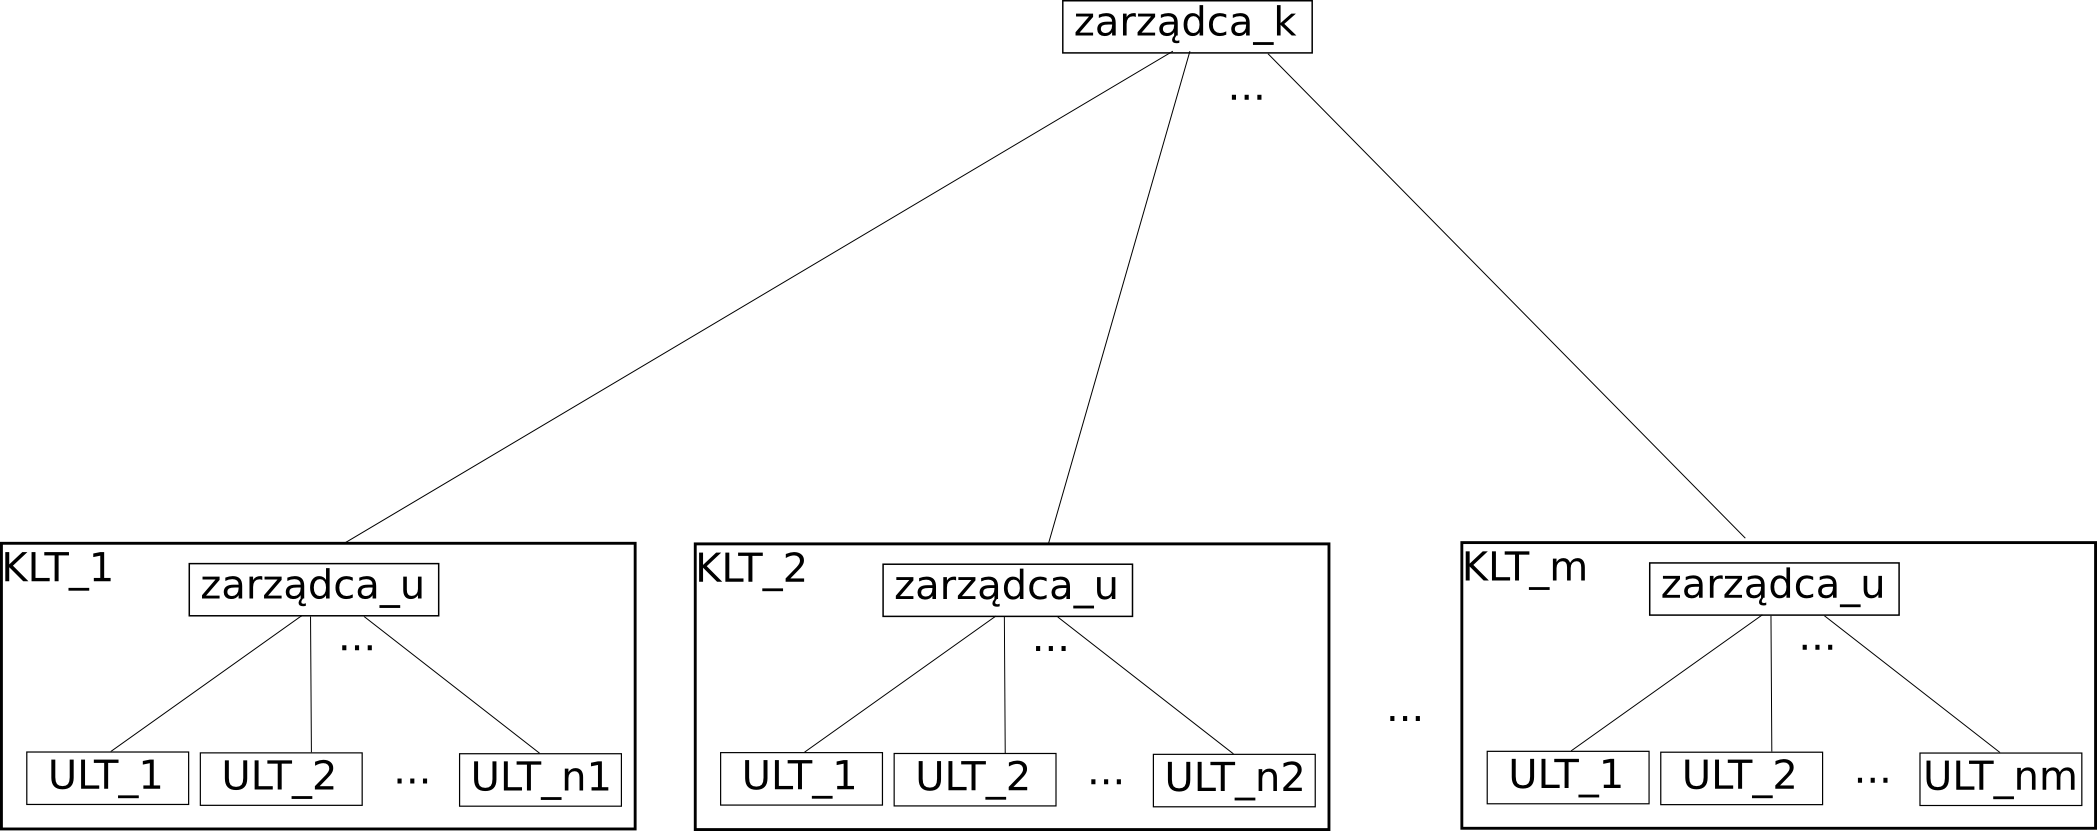
\includegraphics[scale=.21]{mixedscheme.png}
		\caption{Schemat implementacji wątków mieszanych alternatywnej do opisanej w~\cite{anderson}
		(KLT: wątek przestrzeni jądra;
			ULT: wątek przestrzeni użytkownika;
			scheduler\_k: zarządca KLT;
			scheduler\_u: zarządca włókien).
		}
	\end{figure}
	Inny pomysł na implementację wątków mieszanych polega na:
	\begin{itemize}
		\item skorzystaniu z~wątków udostępnianych przez jądro: ich liczba może być zależna od ilości dostępnych procesorów w~komputerze
			lub od preferencji użytkownika. Wątki te będą swego rodzaju \emph{pojemnikami}, zaś każdy z~takich wątków będzie zawierać pewną
			liczbę wątków przestrzeni użytkownika (zarządzanych lokalnie wewnątrz każdego pojemnika). Taki schemat wątków hybrydowych pokazany jest na
			rysunku \ref{fig:mixedintro}.
		\item Wątek przestrzeni użytkownika (\emph{włókno}) jest wykonywany w~konkretnym wątku przestrzeni jądra, z~tym zaś jest związany
			konkretny planista włókien, który zarządza ich wykonaniem. Można więc utożsamiać konkretnego planistę włókien z~odpowiadającym mu
			wątkiem przestrzeni jądra.
		\item włókna mogą \emph{wędrować} pomiędzy wątkami przestrzeni jądra, jednak w~danym momencie może nimi zarządzać dokładnie jeden
			planista włókien.
		\item istnieje jeden planista wątków przestrzeni jądra, który zajmuje się komunikacją pomiędzy planistami włókien (wędrówka włókien,
			przesyłanie komunikatów, synchronizacja).
	\end{itemize}
	Jak łatwo zauważyć, taka implementacja może być zaimplementowana jako biblioteka, a~więc nie występuje potrzeba zmieniania jądra systemu operacyjnego.
	Dodatkowym atutem takiego rozwiązania jest możliwość wyboru przez użytkownika, czy chce skorzystać z~wątków mieszanych, czy może tylko z~wątków
	przestrzeni jądra.
\par
%
\subsection{Cel pracy}
\indent
	Celem niniejszej pracy było utworzenie biblioteki wątków mieszanych
	w~języku C++.
	Powinna ona odpowiadać za:
	\begin{enumerate}
		\item Zarządzanie wątkiem mieszanym:
		\begin{itemize}
			\item tworzenie i~destrukcja wątku;
			\item przydział kontekstu wykonania (stosu) dla wątku;
			\item przydział wątku do procesora;
			\item uruchomienie wątku, wstrzymanie wątku (tzn. w~momencie wykonania operacji {\tt yield} przez wątek);
			\item prawidłowa reakcja na wystąpienie wyjątku w~trakcie działania wątku.
		\end{itemize}
		\item Komunikacja:
		\begin{itemize}
			\item wysyłanie i~obsługa komunikatów (po stronie zarządcy i~wątku);
			\item zdarzenia i~sygnały: detekcja wystąpienia, propagacja, obsługa.
		\end{itemize}
		\item \label{itm:communication} Abstrakcja dla urządzeń wejścia\dywiz wyjścia (ang. \emph{jacketing}):
		\begin{itemize}
			\item nieblokujący dostęp do urządzeń (z~punktu widzenia zarządcy wątków);
			\item blokujący i~nieblokujący dostęp do urządzeń (z~punktu widzenia wątku).
		\end{itemize}
		\item \label{itm:shared} Zasoby współdzielone i~synchronizacja wątków:
		\begin{itemize}
			\item wzajemne wykluczanie (ang. \emph{mutual exclusion, mutex});
			\item sekcja krytyczna;
			\item semafory;
			\item warunki i~zmienne warunkowe;
			\item spotkania (ang. \emph{rendezvous});
			\item skrzynka pocztowa (kolejka komunikatów, ang. \emph{message queue}).
		\end{itemize}
		\item Zarządzanie kolejnością i~czasem wykonania wątków (ang. \emph{scheduling}):
		\begin{itemize}
			\item bez stosowania priorytetów (\emph{round\dywiz robin});
			\item przy zastosowaniu priorytetów.
		\end{itemize}
	\end{enumerate}
\par
%
\indent
	Punkty \ref{itm:communication} oraz \ref{itm:shared} opisują tradycyjne podejście do zasobów udostępnianych wątkom, jak również
	komunikację między nimi. Istnieją jednak inne polityki obsługi wątków i~procesów, z~których warto wymienić stworzony w~latach 70. XX wieku 
	\emph{model aktorów} (ang. \emph{actor model}), po raz pierwszy opisany w~\cite{Hewitt1973ActorFormalism}, używany obecnie z~powodzeniem m. in. w~takich językach jak Erlang czy Scala(\cite{scala1}, \cite{scala2}).
	Wykorzystanie tego modelu wydaje się być atrakcyjną alternatywą zarówno dla tradycyjnych implementacji jacketingu, zaś
	użycie go do synchronizacji wątków może okazać się bardziej intuicyjne dla użytkownika niż zastosowanie mechanizmów wymienionych
	w~punkcie~\ref{itm:shared}.
\par
%
\subsection{Streszczenie pracy}
\indent
	\begin{itemize}
	\item[Rozdział \ref{sec:architecture}] opisuje architekturę współczesnego komputera klasy PC. Opis ten koncentruje się na 
		mechanizmach umożliwiających równoległe wykonanie części lub całych rozkazów procesora oraz na zwiększeniu liczby procesorów
		w~komputerze w~celu podniesienia wydajności obliczeń. Poruszone problemy związane z~pamięcią operacyjną jak również opis połączenia
		poszczególnych elementów komputera między sobą, uzasadniają potrzebę projektowania oprogramowania, które będzie wykonywane równolegle.
	\item[Rozdział \ref{sec:system}] opisuje zgrubnie współczesne systemy operacyjne, jak również zarządzanie procesami. Ponieważ wątki są 
		uruchamiane w~ramach procesów, znajomość podstawowych pojęć wymienionych w~tym rozdziale jest pomocna w~zrozumieniu ograniczeń wątków.
	\item[Rozdział \ref{sec:threads}] opisuje wady i~zalety wątków przestrzeni użytkownika oaz przestrzeni jądra. Dodatkowo, zostały w~nim
		opisane powszechnie znane implementacje wątków hybrydowych.
	\item[Rozdział \ref{sec:solution}] opisuje implementację wątków mieszanych opartą na pomyśle opisanym we wstępie.
	\item[Rozdział \ref{sec:analysis}] określa wartość tej implementacji: jej użyteczność oraz wydajność.
	\item[Rozdział \ref{sec:summary}] podsumowuje wykonanie założeń opisanych we wstępie, jak również wyznacza możliwe drogi rozwoju
		powstałej implementacji
	\end{itemize}
\par
%
\section{Architektura systemów komputerowych}
%
\label{sec:architecture}
\indent 
	W~systemie komputerowym (lub w~skrócie: komputerze) można wyróżnić trzy podstawowe składowe:
	\begin{itemize}
		\item procesor (jednostka centralna, CPU): kontroluje działanie komputera, wykonuje operacje na danych;
		\item pamięć główna: przechowuje dane oraz programy. Pamięć w~tym kontekście jest z~natury ulotna (po wyłączeniu komputera,
			jej zawartości nie można odzyskać); jeśli w~treści dokumentu pojawi się słowo \emph{pamięć}, odwoływać się będzie ono do
			pamięci głównej;
		\item urządzenia zewnętrzne (peryferia, I/O): służą do wymiany danych pomiędzy komputerem i~światem zewnętrznym.
	\end{itemize}
	Komunikacja pomiędzy nimi odbywa się za pośrednictwem szyny systemowej (ang. \emph{system bus}).
	Poniższe podrozdziały informują o~podstawowych składnikach systemu komputerowego. Dokładny opis architektury współczesnych
	systemów komputerowych można znaleźć w~\cite{hennessy}.
\par
%
\subsection{Procesor}
%
\indent
	Procesor jest urządzeniem, które posiada:
	\begin{itemize}
		\item własny zestaw instrukcji (zwanych również rozkazami): ich liczba może wynosić od kilkunastu (architektura RISC, 
			ang. \emph{Reduced Set Instruction Computers}) do kilkuset (architektura CISC, ang.
			\emph{Complex Instruction Set Computers}). Często pojedynczy rozkaz posiada wiele trybów adresowania: jako argument
			może użyć własnego rejestru (tryb implikowany), komórki pamięci (tryb bezpośredni), komórki pamięci, której adres został wyliczony
			(tryby: pośredni, pośredni preindeksowany, pośredni postindeksowany). Połączenie instrukcji wraz z~ich trybami adresowania daje 
			stosunkową liczbę rozkazów.
		\item wewnętrzne komórki pamięci, zwane \emph{rejestrami}.
		\item Licznik rozkazów (ang. \emph{program counter}): wyróżniony rejestr, który wskazuje adres następnej instrukcji. 
			Jeśli w~wyniku ostatniej instrukcji następuje skok (warunkowy lub bezwarunkowy), zmieniana jest wartość tego rejestru.
		\item mechanizm \emph{przerwań}: szyna systemowa może w~pewnych sytuacjach poinformować o~wystąpieniu określonego zdarzenia.
			Przerwania można podzielić na maskowalne (procesor zignoruje informację o~wystąpieniu danego zdarzenia) oraz niemaskowalne.
			Przerwania mogą posiadać priorytety (przerwanie o~niższym priorytecie zostanie zignorowane podczas obsługiwania przerwania
			o~wyższym priorytecie lub jego obsługa rozpocznie się po zakończeniu obecnie obsługiwanego przerwania).
	\end{itemize}
\par
%
\indent
	Procesor przetwarza rozkazy. Można podzielić je na pięć grup:
	\begin{itemize}
		\item odczyt / zapis: wczytanie zawartości komórki pamięci do rejestru, zapis zawartości rejestru do komórki;
		\item skoki: bezwarunkowe, warunkowe, pośrednie;
		\item operacje logiczne: NOT, AND, OR, XOR;
		\item arytmetyka: suma, różnica, iloczyn, iloraz;
		\item zmiana stanu procesora: maskowanie przerwań, ustawienie / wyczyszczenie flagi przeniesienia.
	\end{itemize}
	Każdy rozkaz jest wykonywany w~określonym czasie, w~zależności od rozkazu wykorzystywane są specyficzne dla danej instrukcji
	jednostki funkcjonale CPU (np. jednostka arytmetyczno\dywiz logiczna dla rozkazów arytmetycznych, lub licznik rozkazów
	dla skoków warunkowych). Czas wykonania jest mierzony w~\emph{cyklach maszynowych}. Należy mieć na uwadze, 
	iż na jeden cykl maszynowy może składać się więcej niż jeden cykl zegarowy, zaś
	producent, informując o~taktowaniu procesora zegarem o~częstotliwości 1 MHz, ma na myśli, że
	w~ciągu sekundy zostanie wykonanych milion cykli zegarowych.
\par
%
\indent
	Wynik wykonania konkretnego rozkazu może powodować zmiany w~rejestrze jednostki centralnej, w~pamięci lub
	też w~urządzeniu zewnętrznym. Co więcej, każdy procesor wykonuje rozkazy w~pewien określony sposób, w~specyficznej dla siebie liczbie kroków.
	Jednakże, dla wszystkich procesorów, możemy wyróżnić podstawowe kroki wykonania rozkazu:
	\begin{enumerate}
	\item Pobranie (ang. \emph{Instruction Fetch, IF}): wymaga komunikacji z~pamięcią.
		Pobrany rozkaz po pobraniu jest gotowy do dalszego przetwarzania.
	\item Dekodowanie (ang. \emph{Instruction Decode, ID}):  liczba bajtów, które należy pobrać, może być zmienna:
		nawet gdy długość rozkazu jest niezmienna (np. 2 bajty), jego argumenty (\emph{opkodów}, ang. \emph{opcode}) mogą być zmiennej długości.
	\item Wykonanie (ang. \emph{Execute, EX}): poszczególne części procesora wykonują działanie w~kolejności określonej przez aktualnie
		wykonywany rozkaz.
	\item Dostęp do pamięci (ang. \emph{Memory Access, MEM}): rozkazy mogą korzystać z~danych zawartych w~komórkach pamięci. Jeśli bieżący rozkaz
		zapisuje do lub odczytuje zawartość pamięci, w~tym kroku jest dokonywana ta operacja.
	\item Zapis (ang. \emph{Write Back, WB}): stan procesora jest aktualizowany o~wynik działania rozkazu.
	\end{enumerate}
\par
%
\indent
	Klasyczne procesory wykonują rozkazy sekwencyjnie. Kolejny rozkaz zostanie wczytany do pamięci dopiero, gdy
	CPU zapisze wynik bieżącego. Do sekwencyjnego wykonywania rozkazów nie potrzeba żadnych dodatkowych mechanizmów,
	jednak w~trakcie wykonania aktywna jest dokładnie jedna składowa procesora, podczas gdy pozostałe są ,,uśpione''
	w~oczekiwaniu na uruchomienie.
	\begin{table}
	\centering
	\begin{tabular}{|c|c|c|c|c|c|c|c|c|c|c|} \hline
	& \multicolumn{5}{c|}{Rozkaz 1} & \multicolumn{5}{c|}{Rozkaz 2}  \\
	\hhline{|~|*{10}-}& IF & ID & {\cellcolor{yellow}{EX}} & MEM & WB & IF & ID & EX & MEM & WB\\ \hline \hline
	Cykl zegara & 1 & 2 & {\cellcolor{yellow}{3}} & 4 & 5 & 6 & 7 & 8 & 9 & 10 \\ \hline
	\end{tabular}\par
	\caption[Sekwencyjne wykonanie dwóch rozkazów]{Sekwencyjne wykonanie dwóch rozkazów. Wyróżniona kolumna odpowiada bieżącemu krokowi wykonania
	rozkazu.
	}
	\end{table}\par
\par
%
\indent
{\bf Zrównoleglenie wykonania programu na poziomie instrukcji}
\par
%
\indent 
	Pomysł na bardziej efektywne wykorzystanie zasobów jednostki centralnej, to użycie \emph{potokowości} (ang. \emph{pipelining}):
	Jeśli wykonanie bieżącego rozkazu zakończyło się dla komponentu, może on wykonać następny rozkaz.
	\begin{table}[h]
	\centering
	\begin{tabular}{|c|c|c|c|c|c|c|c|} \hline
	Numer 		 & \multicolumn{7}{c|}{\multirow{2}{*}{Stan potoku}} \\
	rozkazu & \multicolumn{7}{c|}{} \\ \hline
	1 & IF & ID & EX & \cellcolor{yellow} MEM & WB & & \\ \hline
	2 & & IF & ID & \cellcolor{yellow} EX & MEM & WB & \\ \hline
	3 & & & IF & \cellcolor{yellow} ID & EX & MEM & WB \\ \hline
	4 & & & & \cellcolor{yellow} IF & ID & EX & MEM \\ \hline
	5 & & & & \cellcolor{yellow} & IF & ID & EX \\ \hline \hline
	Cykl zegara & 1 & 2 & 3 & \cellcolor{yellow} 4 & 5 & 6 & 7 \\ \hline
	\end{tabular}
	\caption[Potokowe wykonanie rozkazów]{Potokowe wykonanie rozkazów. W~kolumnach umieszczone są komponenty wykonujące dany krok rozkazu.
	W~wyróżnionej kolumnie można odczytać, że w~czwartym cyklu zegarowym pierwszy rozkaz jest w~trakcie wykonywania kroku MEM, 
	dla drugiego wykonywany jest krok EX, itd.}
	\label{tab:pipeline}
	\end{table}
	Metoda ta pozwala na ,,równoległe'' wykonanie kilku rozkazów na jednym procesorze, w~przykładzie opisanym w~tabeli \ref{tab:pipeline}, po upływie 7 cykli
	zostaną wykonane trzy rozkazy. Gdyby rozkazy te były wykonane na jednostce sekwencyjnej, czas ich wykonania byłby ponad dwa razy dłuższy.
\par
%
\indent
	Architektura procesora, która jest uogólnieniem potokowości to \emph{Superskalarność} (ang. \emph{Superscalar}): 
	każdemu krokowi odpowiada co najmniej jeden potok, jednakże występuje redundancja części funkcjonalnych procesora.
	\begin{table}[h]
	\centering
	\begin{tabular}{|c|c|c|c|c|c|c|c|} \hline
	Numer 		 & \multicolumn{7}{c|}{\multirow{2}{*}{Stan potoku}} \\
	rozkazu & \multicolumn{7}{c|}{} \\ \hline
	1 & IF & ID & EX & \cellcolor{yellow} MEM & WB & & \\ \hline
	2 & IF & ID & EX & \cellcolor{yellow} MEM & WB & & \\ \hline
	3 & & IF & ID & \cellcolor{yellow} EX & MEM & WB & \\ \hline
	4 & & IF & ID & \cellcolor{yellow} EX & MEM & WB & \\ \hline
	5 & & & IF & \cellcolor{yellow} ID & EX & MEM & WB \\ \hline
	6 & & & IF & \cellcolor{yellow} ID & EX & MEM & WB \\ \hline
	7 & & & & \cellcolor{yellow} IF & ID & EX & MEM \\ \hline
	8 & & & & \cellcolor{yellow} IF & ID & EX & MEM \\ \hline
	9 & & & & \cellcolor{yellow} & IF & ID & EX \\ \hline
	10 & & & & \cellcolor{yellow} & IF & ID & EX \\ \hline \hline
	Cykl zegara & 1 & 2 & 3 & \cellcolor{yellow} 4 & 5 & 6 & 7 \\ \hline
	\end{tabular}
	\caption[Potokowe wykonanie 10 rozkazów na jednostce superskalarnej]
					{Potokowe wykonanie 10 rozkazów na jednostce superskalarnej o~dwóch potokach rozkazów: rozkazy o~numerach nieparzystych są wykonywane na 
					pierwszej jednostce, zaś rozkazy o~numerach parzystych na drugiej. Analogicznie jak w~tabeli \ref{tab:pipeline}, wyróżniona
					kolumna odpowiada wykonaniu programu w~czwartym cyklu zegarowym.}
	\end{table}
	Jak łatwo zauważyć, superskalarny CPU jest w~stanie przetworzyć nawet wektor instrukcji. Warunkiem koniecznym do osiągnięcia takiego
	wyniku jest brak zależności pomiędzy wynikiem wcześniejszej a~następnej instrukcji.
\par
%
\indent
	Opisane wyżej techniki napotykają jednak na podstawowy problem: w~momencie, gdy bieżącym rozkazem jest skok warunkowy, kolejna wczytana 
	instrukcja nie musi być koniecznie kolejną instrukcją programu. Tak więc, częściowo wykonana instrukcja (lub, w~przypadku jednostek
	superskalarnych, nawet w~pełni wykonane rozkazy) nie powinna wywrzeć wpływu na żaden z~zasobów komputera, 
	a~dodatkowo jest ona niepotrzebnie przetwarzana.
\par
%
\indent
	W~celu zniwelowania niedogodności związanych z~,,nietrafionymi'' skokami warunkowymi, zaczęto stosować technikę 
	\emph{przewidywania skoku} (ang. \emph{branch prediction}): stosowane są heurystyki, które określają najbardziej prawdopodobny
	wynik instrukcji skoku. Dzięki stosowaniu tych heurystyk, udaje się w~dużej liczbie przypadków uniknąć niepotrzebnych obliczeń,
	a~wykonywane są te rozkazy, które rzeczywiście są potrzebne do wykonania programu.
	Przewidywanie skoku jest jedną z~technik stosowanych w~mechanizmie zwanym \emph{Wykonaniem spekulatywnym} (ang. \emph{Speculative execution}):
	wykonanie spekulatywne dopuszcza również wykonanie (przy spełnieniu określonych założeń) części programu znajdującego się za skokiem warunkowym,
	ale jeszcze \emph{przed} wykonaniem tego skoku.
\par
%
\indent
	Technika wykonania określonego fragmentu kodu źródłowego jest stosowana również w~mechanizmie \emph{Wykonania poza kolejnością}
	(ang. \emph{Out of Order execution, OoO}): jeśli pewien rozkaz używa wartości rejestru, która została już obliczona, to można go wykonać
	poza kolejnością podaną przez autora programu. Dla sekwencji rozkazów z~rys.~\ref{fig:oooex}
	można zauważyć, że rozkaz (3) korzysta z~wartości rejestru A3, który jest wyliczony w~(1), jego wykonanie nie ma wpływu na rejestry, z~których 
	korzysta (2), a~więc sekwencja $\langle 1, 3, 2 \rangle $ da po wykonaniu wynik taki sam, jak sekwencja $\langle 1, 2, 3 \rangle $.
	\begin{figure}[h]
	\begin{tabular}{l}\\
		(1) {\tt add A1,A2,A3 /* dodaj A1 do A2, wynik zapisz do A3 */ } \\
		(2) {\tt add A1,A4,A5 } \\
		(3) {\tt add A2,A3,A7 } \\
		\\
	\end{tabular}
	\caption{Wykonanie poza kolejnością}
	\label{fig:oooex}
	\end{figure}
\par
%
\indent
	Podczas wykonania programu pewne rejestry procesora są wykorzystywane częściej, zaś inne rzadziej. Aby zwiększyć użycie rzadziej
	używanych rejestrów i~wykonać kolejne rozkazy poza kolejnością, można tymczasowo potraktować nieużywany rejestr jak ten, który miał
	być pierwotnie użyty do wykonania rozkazu (zapisać jego dotychczasową wartość, skopiować wartość z~odpowiedniego rejestru, wykonać instrukcję,
	przywrócić poprzednią wartość tak wykorzystanego rejestru). Taka technika jest zwana 
	\emph{Przemianowaniem rejestrów} (ang. \emph{Register Renaming}).
\par
%
\indent
	Dzięki opisanym wyżej technikom możliwe jest zrównoleglenie wykonania programu (w~stosunku do procesora wykonującego rozkazy sekwencyjnie)
	już na poziomie pojedynczych instrukcji procesora. Stąd też techniki te są określane mianem \emph{instruction level parallelism} (ILP).
	Podstawową zaletą tych technik jest znaczące przyspieszenie działania procesora, jednakże implementacja tych technik w~procesorze pociąga za
	sobą zwiększenie liczby tranzystorów, a~co za tym idzie, zwiększenie temperatury wydzielanej przez CPU.
\par
%
\indent
	Problemem, który jest naturalnie związany z~ILP to zależność od danych (ang. \emph{data dependency}).
	Dotyczy on zachowania oryginalnej chronologii wykonywania rozkazów (zapisu wyników
	ich działania w~procesorze, pamięci i~urządzeniach zewnętrznych). W sekwencji przedstawionej na rys.\ref{fig:datadep}
	\begin{figure}[h]
	\begin{tabular}{l l}\\
		(1) & {\tt add Y,Z,X} \\
		(2) & {\tt add U,V,T} \\
		(3) & {\tt mult X,T,L /* zapisz iloczyn X}$\times${\tt T do L */} \\
		(4) & {\tt add L,T,L} \\
	\end{tabular}
	\caption{Ilustracja problemu zależności od danych}
	\label{fig:datadep}
	\end{figure}
	instrukcje (1) i~(2) mogą wyć wykonane w~kolejności $\langle 1,2 \rangle$ jak i~$\langle 2,1 \rangle$, zaś wynik działania instrukcji
	(3) zależy bezpośrednio od wyników działania (1) i~(2). Co więcej, instrukcja (4) nie może być wykonana wcześniej 
	niż po zakończeniu wykonania instrukcji (1), (2) i~(3). Tak więc chronologia wykonania instrukcji (3) i~(4) nie może być zmieniona.
\par
%
\indent
	W~celu rzeczywistego zrównoleglenia działania programu, w~komputerach pojawiło się więcej procesorów,
	które działały niezależnie od siebie. Procesory były pojedynczymi układami, bądź kilka procesorów umieszczano w~jednym układzie. 
	Pojedynczy procesor w~kości zawierającej kilka jednostek centralnych zwany jest \emph{rdzeniem} (ang. \emph{core}).
	Odpowiednio zaprojektowany program,	który korzysta z~kilku procesorów może przyspieszyć swoje działanie nawet proporcjonalnie do ich liczby,
	na których jest wykonywany.	Takie przyspieszenie działania programu, choć możliwe, jest rzadko spotykane.
	Dobrą ilustracją problemu przyspieszania działania procesora jest prawo Amdahla, opisane w~dalszej części tego dokumentu.
\par
%
\indent
	Michael J.~Flynn stworzył klasyfikację systemów komputerowych oraz programów (\emph{taksonomia Flynna}), w~której ze względu na liczbę
	strumieni rozkazów oraz danych, wyróżniamy cztery klasy, wymienione w~tabeli \ref{tab:flynn}.
	\begin{table}[h]
	\centering
	\begin{tabular}{|c|c|c|} \hline
													 & Jeden strumień instrukcji	 & Wiele strumieni instrukcji \\
													 & (\emph{Single Instruction}) & (\emph{Multiple Instruction}) \\\hline
			Jeden                &     												 &      \\
			strumień danych      &  SISD										   & MISD 			\\
			(\emph{Single Data}) &                             & \\\hline
			Wiele                &     												 &      \\
			strumieni danych     & SIMD                        & MIMD \\
			(\emph{Multiple Data}) & 										 & 			\\\hline
	\end{tabular}
	\caption{Taksonomia Flynna}
	\label{tab:flynn}
	\end{table}
	Klasy te możemy scharakteryzować w~następujący sposób:
	\begin{itemize}
		\item SISD jest klasą programów wykonywanych sekwencyjnie na maszynie sekwencyjnej;
		\item SIMD odpowiada programom wykonywanym na maszynie superskalarnej lub na procesorach przetwarzających sygnały (DSP);
		\item MISD jest klasą maszyn i~programów, która ma zastosowanie tam, gdzie liczy się minimalizacja błędów;
		\item MIMD odpowiada programom wykonywanym na wielu procesorach.
	\end{itemize}
\par
\indent
	Komputery sklasyfikowane jako MIMD, ze względu na rodzaj komunikacji pomiędzy procesorami, można podzielić na dwie podklasy:
	\begin{itemize}
		\item o~rozproszonej pamięci: każdy procesor posiada przyporządkowaną
			dla niego pamięć. W~takim układzie procesory wraz z~pamięcią im dedykowaną mogą być traktowane jako oddzielne komputery, 
			zaś komunikacja między nimi przebiega po pewnej ustalonej ścieżce (np. za pomocą połączenia sieciowego).
			Taka architektura systemu komputerowego nazywana jest \emph{wieloprocesorowością asymetryczną} (ang. \emph{asymmetric multiprocessing, AMP}),
			zaś najczęściej jest spotykana w~systemach rozproszonych czy klastrach.
		\item o~dzielonej pamięci: wszystkie procesory korzystają z~tej samej pamięci.
	\end{itemize}
	W~systemach, w~których wszystkie procesory korzystają z~jednej, dzielonej pamięci, komunikacja pomiędzy procesorami odbywa się za jej pomocą.
	Można wyróżnić dwie najczęściej stosowane architektury:
	\begin{itemize}
		\item nadrzędna jednostka/jednostka podrzędna (ang. \emph{master/slave}): jeden z~procesorów posiada uprzywilejowany dostęp do pamięci (master).
			Na tym procesorze są wykonywane najważniejsze dla programu zadania (np. \emph{jądro systemu operacyjnego}, ang. \emph{kernel}),
			zaś pozostałe jednostki centralne posiadają ograniczony dostęp do pamięci (slave), jak również do innych zasobów komputera 
			(np. aplikacje użytkownika systemu operacyjnego).
			Jeśli jednostka podrzędna potrzebuje wykonania pewnego działania, które może być wykonane jedynie przez jednostkę nadrzędną, musi w~tym celu
			przesłać żądanie do jednostki typu master. Taka architektura posiada dwie zasadnicze wady:
			\begin{itemize}
				\item błąd (usterka) jednostki uprzywilejowanej powoduje zerwanie działania programu (systemu operacyjnego);
				\item jednostka typu master może stać się \emph{wąskim gardłem} (ang. \emph{bottleneck}) programu (systemu operacyjnego),
					gdy ilość żądań wykonania specyficznych dla niej operacji przekroczy pewien zależny od niej samej próg, lub też gdy pewne
					operacje będą wykonywane w~sposób nieefektywny.
			\end{itemize}
		\item \emph{SMP} (ang. \emph{symmetric multiprocessing}): wszystkie procesory w~systemie komputerowym posiadają identyczne przywileje
			dostępu do pamięci oraz innych jego zasobów. Dzięki temu, możliwe jest wykonywanie jednej aplikacji na wielu procesorach jednocześnie,
			możliwa jest również ,,wędrówka'' wydzielonych części aplikacji po wszystkich dostępnych w~komputerze procesorach.
	\end{itemize}
\par
%
\indent
	Opisane powyżej techniki stosowane w~architekturach procesorów, jak również same architektury systemów operacyjnych, kładą nacisk na
	zrównoleglenie wykonywania programów. Głównym wyzwaniem, jakie stoi przed programistą, jest takie zaprojektowanie aplikacji,
	aby można było ją wykonać równolegle na jak największej liczbie procesorów, co przełoży się na krótszy czas wykonania.
	Aplikacja będzie komunikować się ze światem zewnętrznym, a~w~szczególności z~użytkownikiem o~wiele sprawniej, niż ta sama aplikacja,
	ale zaprojektowana w~sposób sekwencyjny.
\par
%
\indent
	Można zauważyć, że wzrost mocy obliczeniowej maszyn wieloprocesorowych (wielordzeniowych) w~stosunku do maszyn klasy SISD (SIMD) jest
	analogiczny do wzrostu mocy obliczeniowej procesora posiadającego architekturę ILP do procesora posiadającego architekturę sekwencyjną.
	Jednakże, aby wykorzystać potencjał architektur równoległych,
	zarówno ILP jak i~MIMD wymagają odpowiednio zaprojektowanych i~zaprogramowanych aplikacji.
\par
%
\subsection{Pamięć}
\indent
	Pamięć w~systemie komputerowym możemy podzielić na dwa rodzaje: ulotną i~trwałą. Informacje znajdujące się w~pamięci ulotnej
	nie będą odzyskane po wyłączeniu i~ponownym włączeniu komputera. Można wyróżnić dwa rodzaje pamięci ulotnej:
	\begin{itemize}
		\item wewnętrzna: procesor komunikuje się z~nią bez pośrednictwa szyny systemowej. Jest taktowana tą samą częstotliwością, co CPU
			(lub bardzo do niej zbliżoną). Pamięciami tego rodzaju są:
			\begin{itemize}
				\item rejestry procesora;
				\item pamięć podręczna (ang \emph{cache}), często wielopoziomowa.
			\end{itemize}
		\item Systemowa (operacyjna): szyna systemowa pośredniczy podczas operacji odczytu/zapisu do pamięci tego rodzaju. Ta pamięć jest zwana
			pamięcią główną komputera (ang. \emph{main memory, primary memory}), a~ponieważ dostęp do każdej komórki tej pamięci
			w~każdym momencie działania systemu komputerowego jest możliwy, zwana jest również pamięcią o~dostępie swobodnym
			(ang. \emph{random access memory, RAM}).
	\end{itemize}
	Z~punktu widzenia procesora, pamięć trwała jest pamięcią ,,za'' szyną systemową, za wyjątkiem pamięci stałej (ang. \emph{read only memory, ROM}),
	nie znajduje się ona nawet na płycie głównej, na której znajduje się jednostka centralna, dlatego pamięci tego rodzaju zwane są 
	zewnętrznymi. O~ile pamięć główna jest uprzywilejowanym urządzeniem o~najszybszym dostępie, o~tyle dostęp do pamięci
	zewnętrznych jest o~wiele wolniejszy. Do trwałych pamięci zewnętrznych zaliczyć można następujące urządzenia:
	\begin{itemize}
		\item dyski magnetyczne (dyskietki, dyski twarde, SSD, pamięci typu Flash);
		\item płyty CD, DVD, BD;
		\item taśmy magnetyczne.
	\end{itemize}
\par
%
\indent
	Występuje następująca hierarchia pomiędzy rodzajami pamięci:
	\begin{enumerate}
		\item pamięć znajdująca się na płycie głównej (ang. \emph{inboard storage}), czyli rejestry, cache, RAM oraz ROM;
		\item pamięć poza płytą główną (ang. \emph{outboard storage}): dyski, płyty CD, DVD, BD;
		\item pamięć niepodłączona (ang. \emph{off\dywiz line storage}), przede wszystkim taśmy magnetyczne,
			na których składowane są dane, ale dostęp do nich jest sporadyczny (dane są zapisywane w~czasie sesji zapisu,
			podobnie limitowany jest odczyt z~tego rodzaju pamięci).
	\end{enumerate}
	Najwyżej w~tej hierarchii stoi pamięć na płycie głównej: z~punktu widzenia procesora, czas dostępu do rejestrów jest natychmiastowy,
	podobnie rzecz ma się z~pamięcią cache. Dostęp do pamięci RAM (ROM) wymaga minimalnie więcej czasu, niż ma to miejsce przy dwóch
	wcześniej wymienionych rodzajach pamięci. Nasuwają się pytania: ,,czy nie lepiej, zamiast pamięci RAM, umieścić całą
	pamięć operacyjną w~kości procesora, rezygnując z~pośrednictwa szyny systemowej\mbox{}? Co jest przyczyną takiej organizacji pamięci ulotnej\mbox{}?''
	Jest kilka odpowiedzi na te pytania:
	\begin{enumerate}
		\item Koszty wytworzenia pamięci. Najdrożej jest wytworzyć pamięć najszybszą przy wymaganej niezawodności oraz szybkości działania.
			Dlatego rejestry procesorach mają rozmiar co najwyżej kilkaset bajtów, cache pierwszego poziomu (ang. \emph{level one cache})
			jest wielkości liczonej w~kilobajtach, cache drugiego (a~także trzeciego) poziomu liczony jest w~megabajtach, zaś
			rozmiar pamięci RAM to kilka (do kilkunastu) gigabajtów.
		\item Technologia, w~jakiej wytwarzane są obecnie pamięci oraz procesory nie pozwala na umieszczenie na jednej kości kilku rdzeni
			wraz z~kilkoma gigabajtami pamięci operacyjnej. Obecnie kości zawierające kilka rdzeni wydzielają bardzo dużo ciepła, a~po dodaniu
			pamięci, taki układ elektroniczny z~powodu wydzielania ciepła byłby bardzo niestabilny. Od roku 2006 można zauważyć,
			że częstotliwość taktowania procesorów nie wzrasta w~takim stopniu, jak to miało miejsce do tego momentu. To także efekt ograniczeń,
			jakie istnieją w~wyniku wydzielania temperatury przez jednostkę centralną.
		\item Modularność. Po wystąpieniu awarii (np. niedziałający bit pamięci), Pamięć operacyjna, będąca urządzeniem zewnętrznym, może zostać
			wymieniona na niewadliwą. W~przypadku umieszczenia pamięci wraz z~procesorem, taka wymiana pociągnęła by za sobą o~wiele większe
			koszty. Co więcej, z~pamięci operacyjnej może korzystać wiele procesorów, które znajdują się w~różnych układach rozsianych po płycie głównej.
			Z~pamięci korzystać mogą również inne urządzenia niż procesor (np. karta graficzna, dyski), więc obsługa żądań tych urządzeń mogła by być
			sporym obciążeniem dla samego procesora. Oczywiście istnieją specjalizowane systemy komputerowe, w~których jedyną dostępną 
			pamięcią operacyjną jest cache (architektura COMA, ang. \emph{cache only memory architecture}).
	\end{enumerate}
\par
%
\indent
	W~powszechnych zastosowaniach używa się architektur pamięci, w~których występuje RAM. Są to:
	\begin{itemize}
		\item pamięć niejednorodna (ang. \emph{non\dywiz uniform memory architecture, NUMA}): każdy procesor posiada własną pamięć operacyjną
			(która nie jest współdzielona z~innymi jednostkami), a~dodatkowo posiada dostęp do pamięci operacyjnej współdzielonej z~innymi CPU.
			Niektóre procesory mogą mieć priorytet w~dostępie do pamięci dzielonej.
		\item Pamięć jednorodna (ang. \emph{uniform memory architecture, UMA}): wszystkie procesory mają dostęp do dzielonej pamięci operacyjnej.
			Każdy z~nich posiada równoprawny dostęp do tej pamięci.
	\end{itemize}
	Powyższe architektury mogą być zastosowane zarówno w~maszynach SMP, jak również w~AMP.
\par
%
\indent
	Pamięci trwałe, znajdujące się poza płytą główną systemu komputerowego, posiadają jedną zasadniczą cechę: ich koszt w~przeliczeniu na jednostkę
	(np. bajt) jest o~wiele niższy niż w~wypadku pamięci znajdującej się na płycie głównej. Okupione jest to znacznie dłuższym czasem dostępu 
	do nich, dlatego w~powszechnym użyciu stosowane jest rozwiązanie polegające na wymianie komunikatów o~pobraniu/przesłaniu danych pomiędzy
	procesorem a~urządzeniem, zaś same dane do tego typu operacji znajdują się w~pamięci RAM i~są tam przesyłane (lub pobierane) przez urządzenie.
	Mechanizm, który umożliwia takie przesyłanie danych zwany jest bezpośrednim dostępem do pamięci (ang. \emph{direct memory access}).
\par
%
\indent
	Pamięci typu off\dywiz line są używane przede wszystkim jako magazyn do przechowywania danych w~ilości przekraczającej rozmiary pamięci trwałej.
	W~porównaniu do pamięci stojących wyżej w~hierarchii, takie pamięci posiadają bardzo duży rozmiar, jednakże czas dostępu do danych w~nich
	zawartych jest liczony w~minutach, lub nawet godzinach.
\par
%
\indent
	Można zauważyć, że ,,murem'' oddzielającym procesor od pamięci (za wyjątkiem pamięci wewnętrznej) jest szyna systemowa.
	Szyny systemowe, w~obecnych komputerach, są taktowane niższymi częstotliwościami (nawet kilkakrotnie), niż sam procesor.
	Także sama pamięć RAM może być taktowana częstotliwością niższą zarówno od wymienionych wcześniej.
	Taka dysproporcja w~taktowaniu części systemu komputerowego może prowadzić do przestojów w~pracy procesora: nie może wykonać żadnego działania,
	ponieważ nie ma kolejnych instrukcji programu! Rosnąca dysproporcja w~taktowaniu procesorów i~pamięci jest zwana \emph{murem pamięciowym}
	(ang. \emph{memory wall}).
\par
%
\indent
	Okazuje się, że wywołanie spekulatywne może być pomocne podczas rozstrzygania problemu pobierania właściwych danych zawierających 
	dane programu. W~celu uniknięcia przestojów jednostki centralnej, stosowany jest również cache dla instrukcji procesora.
\par
%
\indent
	Pamięć podręczna jest bardzo ważną częścią pamięci ulotnej: to z~tej pamięci (a~dokładniej: z~pamięci pierwszego poziomu) procesor
	może pobierać pojedyncze bajty i~tylko na tej pamięci może on wykonywać operacje odczytu/zapisu. 
	Z~pamięci RAM dane pobierane są do pamięci cache (do najwyższego poziomu cache\dywiz u) w~paczkach o~określonej wielkości (np. 32 bajty),
	dzięki czemu zmniejsza się liczba żądań dostępu pamięci podręcznej (widzianej przez szynę danych jako procesor) do pamięci operacyjnej.
	Takie rozwiązanie pociąga za sobą problem zgodności danych: jeśli procesor zmieni zawartość pewnej komórki pamięci,
	to zawartość odpowiadającej jej komórki w~pamięci operacyjnej powinna być taka sama w~momencie odczytu dokonywanego przez inny procesor
	znajdujący się w~systemie. Problem ten można rozwiązać na dwa sposoby:
	\begin{itemize}
		\item jeśli zgłaszane jest żądanie dostępu do komórki przez rdzeń znajdujący się w~tym samym układzie, wystarczy wymienić wartość komórki
			tylko we współdzielonej pamięci podręcznej, a~następnie przesłać ją do cache\dywiz u~pierwszego poziomu, do którego dostęp posiada
			rdzeń, który zgłosił żądanie. Zawartość pamięci operacyjnej zostanie uaktualniona \emph{później}.
		\item Jeśli dostępu do komórki zażądał inny procesor, wówczas należy przesłać zawartość komórki do pamięci RAM.
	\end{itemize}
	Oczywiście, jeśli następuje zmiana zawartości pamięci podręcznej, zawartość zmienionej komórki musi zostać przesłana do pamięci operacyjnej
	(jest to sytuacja, która została określona jako ,,później'').
\par
%
\indent
	Powyższy opis zastosowania pamięci podręcznej pozwala uzmysłowić intensywność jej użycia, a~także jej niebanalne we współczesnych
	systemach komputerowych: tworząc jakikolwiek program, dobrze jest mieć na uwadze rozmiary pamięci cache, 
	gdyż jeśli program będzie wykonywać operacje na komórkach pamięci, bardzo często będzie dochodzić wtedy do \emph{rozminięcia} zawartości
	cache\dywiz u z~żądanymi danymi, które procesor będzie musiał pobierać z~pamięci operacyjnej (ang. \emph{cache miss}), co zaowocuje
	długimi przestojami w~pracy procesora, a~w~konsekwencji może doprowadzić do spadku wydajności aplikacji. Obniżenie liczby nietrafionych 
	żądań dostępu do tych trafionych (ang. \emph{cache hit}) może skutkować sprawnie działającą aplikacją.
\par
%
\indent
	Dokładny i~wyczerpujący opis pamięci stosowanych we współczesnych komputerach można znaleźć w~\cite{jacob}.
\par
%
\subsection{Urządzenia zewnętrzne}
\indent
	Urządzenia zewnętrzne, znane również jako \emph{peryferia}, \emph{urządzenia wejścia\dywiz wyjścia}, \emph{I/O} (\emph{ang. Input/Output}),
	to, oprócz pamięci trwałych, także urządzenia do komunikacji komputera ze światem zewnętrznym. 
	Można podzielić je według właściwości odczytu/zapisu na trzy grupy:
	\begin{itemize}
		\item{tylko odczyt danych, np.} klawiatura, mysz, 
		\item{tylko zapis, np.} wyświetlacz,
		\item{odczyt i~zapis, np.} karta sieciowa, graficzna, dźwiękowa, \ldots
	\end{itemize}
\par
%
\indent
	Komunikacja procesora z~peryferiami odbywa się poprzez szynę systemową. Sposób połączenia tych urządzeń z~szyna systemową może się różnić
	i~być jednym z~podanych:
	\begin{itemize}
		\item procesor oraz wszystkie peryferia są podłączone do jednej szyny systemowej. Możliwa jest komunikacja pomiędzy różnymi urządzeniami
			w~systemie komputerowym. Takie połączenie urządzeń wymusza uczestnictwo procesora w~wymianie danych z~I/O.
		\item Procesor oraz pamięć operacyjna podłączone są do szyny systemowej, zaś pozostałe urządzenia są podłączone do jednostki bezpośredniego
			dostępu do pamięci. Taka architektura systemu komputerowego może być zorganizowana na dwa sposoby:
			\begin{itemize}
				\item DMA jest jednym urządzeniem podłączonym do szyny systemowej, do którego współdzielony dostęp posiadają wszystkie urządzenia
					zewnętrzne. Komunikacja pomiędzy peryferiami a~DMA odbywa się przy użyciu \emph{szyny wejścia\dywiz wyjścia} 
					(ang. \emph{I/O bus}).
				\item Istnieje wiele urządzeń DMA, podłączonych do szyny systemowej, a~grupy urządzeń podłączonych do każdego z~nich mają do niego
					bezpośredni dostęp.
			\end{itemize}
	\end{itemize}
\par
%
\indent
	Komunikacja pomiędzy procesorem, a~peryferiami jest rozwiązana dwojako:
	\begin{itemize}
		\item bez użycia przerwań: stosuje się wówczas technikę \emph{aktywnego czekania} (ang. \emph{busy waiting}). Metoda ta
			wymaga od procesora nieustannego sprawdzania stanu urządzeń. W~razie zmiany stanu urządzenia, podejmowana jest odpowiednia
			akcja, stosowna do rodzaju zdarzenia, jak i~urządzenia.
		\item Stosowany jest mechanizm przerwań. Zmiana stanu urządzenia wejścia\dywiz wyjścia powoduje wysłanie sygnału,
			który wyzwala określone przerwanie \linebreak 
			w~procesorze: wykonanie dotychczasowych instrukcji jest zawieszane, a~uruchamiana jest
			procedura obsługi danego przerwania. Można wyróżnić dwa sposoby przesyłania danych pomiędzy procesorem a~I/O:
			\begin{itemize}
				\item procesor, po uprzednim pobraniu danych, przesyła je do urządzenia. Ponieważ przesyłanie dużych ilości danych w~niedużych
					porcjach (np. bajt) powodowało by bardzo dużą liczbę przerwań oraz duży narzut czasowy na ich pobieranie z~pamięci operacyjnej,
					do takiego rodzaju przesyłania danych stosuje się \emph{bufory}, zawierające większą porcję danych, które są przesyłane 
					na raz do urządzenia zewnętrznego. W~zależności od potrzeb, bufor może być pojedynczym blokiem pamięci, może składać się 
					z~kilku bloków z~wyróżnionym blokiem do przesłania (jak również może być to blok, który zostanie zapełniony danymi przesłanymi
					z~urządzenia peryferyjnego) do I/O w~danym momencie, a~aktualny blok jest wybierany cyklicznie z~puli dostępnych. W~zależności
					od potrzeb oraz możliwości systemu komputerowego, kształt bufora jest określany przez politykę obsługi I/O oraz dostępne 
					mechanizmy, które można zastosować.
				\item Procesor jest informowany o~wystąpieniu zdarzenia w~urządzeniu I/O (lub sam wysyła do niego odpowiedni komunikat), zaś
					dane są przesyłane przez DMA bezpośrednio z~pamięci do odpowiedniego urządzenia, bądź w~kierunku przeciwnym.
					Rozwiązanie to wymaga od procesora jedynie reakcji na zdarzenie, zaś transfer danych odbywa się bez jego udziału.
			\end{itemize}
	\end{itemize}
	Jak można zauważyć, przy użyciu DMA udział procesora w~komunikacji z~peryferiami ograniczony jest do absolutnego minimum. Dlatego też
	komunikacja większości urządzeń I/O z~procesorem odbywa się za jego pośrednictwem.
\par
%
\newpage
\section{System operacyjny}
%
\label{sec:system}
\indent
	System operacyjny (ang. \emph{operating system, OS}, zwany dalej \emph{systemem}) jest programem, 
	który kontroluje wykonanie aplikacji użytkownika (programów),
	może być postrzegany jako pośrednik (interfejs) pomiędzy aplikacją a~sprzętem (systemem komputerowym), na którym jest wykonywany.
	Musi spełniać następujące warunki:
	\begin{itemize}
		\item wygoda: system sprawia, że komputer jest wygodny w~użyciu;
		\item wydajność: system wydajnie zarządza zasobami komputera;
		\item rozszerzalność: OS powinien być zaprojektowany w~sposób umożliwiający łatwe rozszerzanie o~kolejne funkcje;
			również usprawnienia dotychczasowych funkcji powinny odbywać się tak, aby zmiany nie zmuszały użytkownika do zmian w~aplikacji
			-- zmiany powinny być dla niego \emph{przezroczyste}.
	\end{itemize}
	Najważniejszą zyskiem z~używania systemu jest możliwość uruchomienia aplikacji na różnych systemach komputerowych, na których
	jest on dostępny, a~więc aplikacja jest \emph{przenośna}.
\par
%
\indent
	Powinnościami systemu operacyjnego są:
	\begin{itemize}
		\item wykonanie programu: aplikacje użytkownika są uruchamiane w~środowisku dostarczanym przez system operacyjny. Środowisko to 
			udostępnia zasoby, których aplikacje te potrzebują. Dodatkowo, OS zarządza kolejnością wykonania tych programów (ang. \emph{scheduling}).
		\item Rozwój aplikacji: OS dostarcza zestaw narzędzi do tworzenia i~rozwijania aplikacji użytkownika począwszy od
			edytorów po kompilatory. Większość aplikacji jest pisana w~językach programowania wysokiego poziomu (o~których szerzej w~dalszej części
			tej pracy), a~to właśnie kompilator odpowiada za generację kodu maszynowego, który zostanie wykonany w~optymalny sposób
			na procesorze (lub procesorach), z~wykorzystaniem ILP.
		\item Dostęp do I/O: system operacyjny jest pośrednikiem pomiędzy programem a~peryferiami. Ze względu na swoją unikalność,
			każde urządzenie zewnętrzne jest unikatowe, lecz system operacyjny przydziela je do odpowiednich klas abstrakcji, dzięki czemu
			użytkownik nie musi na przykład dbać o~to, czy dane pochodzą z~dysku twardego, posiadającego obracające się talerze a~odczyt/zapis danych
			jest wykonywany za pomocą głowic, czy może urządzeniem tym jest dysk SSD posiadający kości pamięci Flash.
		\item Kontrolowany dostęp do plików: dane składowane w~pamięciach zewnętrznych składowane są w~postaci \emph{plików} (ang. \emph{files}).
			Jest to konsekwencją ogromnego rozmiaru pamięci zewnętrznych (w~porównaniu do pamięci operacyjnej). Dodatkowo, dane te muszą być przedstawione
			człowiekowi w~zrozumiałej formie. Dlatego też powstała idea systemu plików (ang. \emph{file system}). Obecnie istnieją rozwiązania, 
			które oferują wytworzenie, w~sposób przezroczysty, systemu plików, który obejmuje zawartość wielu (często rozproszonych) systemów plików.
			OS może uznać, że dana aplikacja \emph{nie powinna} używać pewnych plików, niektóre z~nich może używać tylko do odczytu, zaś pewne z~nich
			może zarówno odczytać, jak również modyfikować. W~tym celu musi posiadać mechanizmy do limitowania dostępu do plików.
		\item Dostęp do systemu: pewne zasoby systemu mogą być używane jedynie przez jego własne komponenty, np. wspomniany wyżej bezpośredni
			(niskopoziomowy, ang. \emph{low\dywiz level}) dostęp do peryferiów. Jak okaże się w~dalszej części tego tekstu, niektóre dane znajdujące się 
			w~pamięci operacyjnej mogą być używane przez dokładnie jedną aplikację; do tego celu stosowany jest mechanizm stronicowania pamięci
			(ang. \emph{memory paging}).
		\item Wykrywanie błędów oraz reakcja na nie: w~trakcie działania systemu operacyjnego może wystąpić sytuacja awaryjna:
		\begin{itemize}
			\item awaria może wystąpić w~jednym z~urządzeń zewnętrznych, np. błąd w~odczycie z~dysku twardego;
			\item jedna z~wykonywanych aplikacji użytkownika może wykonać niedozwoloną operację, np. próba niedozwolonej operacji na pewnym zasobie;
			\end{itemize}
			w~takiej sytuacji OS musi zareagować stosownie do wykrytego błędu, np. poinformować aplikację o~niemożności odczytu danych z~dysku, lub
			poinformowanie o~braku dostępu do zasobu.
		\item Księgowanie: śledzenie zachowania aplikacji, wytwarzanie bazy informacji, a~następnie ich analiza może dać efekt w~postaci
			nowej wersji systemu, która, przy uwzględnieniu wniosków płynących z~analiz, będzie w~większym stopniu odpowiadać wymaganiom aplikacji,
			a~co za tym idzie, spowoduje szybsze działanie systemu. Większość współczesnych systemów operacyjnych posiada określone zastosowania
			(np. system Windows 7 wykonywany jest dla jednego użytkownika, który pracuje na jednej stacji roboczej, zaś system GNU/Linux
			powinien w~założeniu obsługiwać wielu użytkowników jednocześnie, niekoniecznie za pomocą interfejsu graficznego), dlatego gromadzenie
			i~analiza informacji o~specyficznych dla tych systemów kombinacjach uruchomionych aplikacji w~danym momencie oraz samym zachowaniu użytkownika,
			może dać efekt w~postaci zwiększenia wydajności najczęściej (najbardziej intensywnie) używanych składowych systemu, nawet kosztem
			zmniejszenia wydajności innych składowych systemu.
	\end{itemize}
\par
%
\indent
	Aplikacje użytkownika wykonywane pod kontrolą systemu operacyjnego mogą być bardzo proste (np. program do zliczania słów w~pliku tekstowym),
	jak również bardzo złożone (program do obsługi transakcji bankowych, który z~powodu spełniania ogromnej liczby wymagań, może być potraktowany jako
	system). OS musi zatem udostępniać pewną abstrakcję systemu operacyjnego, która udostępni aplikacji wszystkie usługi oraz zapewni swego
	rodzaju iluzję wyłączności dostępu do zasobów systemu (umożliwiając jednocześnie komunikację z~innymi aplikacjami).
	Tą abstrakcją jest \emph{proces} (ang. \emph{process}).
\par
%
\indent
	Ze względu na dostęp do zasobów komputera, procesy uruchomione przez system operacyjny można podzielić 
	na dwie zasadnicze grupy (warstwy), które z~punktu widzenia procesów są traktowane jak środowisko, w~którym działają 
	(lub są ich \emph{przestrzeniami}): 
	\emph{przestrzeń jądra} (ang. \emph{kernel space}) oraz \emph{przestrzeń użytkownika} (ang. \emph{user space}).
\par
%
\indent
	Jądro systemu to jego podstawa, która jest odpowiedzialna za zarządzanie jego usługami, jak również zasobami, m. in. pamięcią, I/O,
	przydzielaniem czasu procesora poszczególnym programom. Instrukcje procesu jądra wykonywane są w~przestrzeni jądra. Dzięki temu,
	mają one dostęp do wszystkich zasobów systemu komputera i~mogą je dowolnie zmieniać. Dlatego też procesy uruchamiane w~przestrzeni
	jądra muszą być zaprojektowane zgodnie ze wszystkimi wymaganiami stawianymi danemu systemowi operacyjnemu, wraz z~podstawowym wymaganiem:
	muszą one być \emph{niezawodne}, gdyż w~razie wystąpienia poważnego błędu w~trakcie wykonywania programu uruchomionego w~przestrzeni jądra,
	działanie wszystkich aplikacji w~systemie zostanie zaburzone, a~w~konsekwencji może doprowadzić to do unicestwienia całego systemu operacyjnego.
	Ze względu na budowę, można wyróżnić dwa rodzaje jądra systemu:
	\begin{itemize}
		\item jądro monolityczne (ang. \emph{monolithic kernel}), które zawiera w~sobie większą część usług systemu. Wszystkie usługi jądra
			wykonywane są w~ramach jednego procesu, co daje w~efekcie prowadzi do wysokiej wydajności działania takiego jądra. Wadą takiego jądra
			jest fakt, że w~momencie błędu w~działaniu jednego z~jego składników, może dojść do załamania pracy całego procesu, a~w~konsekwencji,
			do załamania pracy całego systemu.
			Przykładem jądra monolitycznego jest jądro systemu Linux, w~którym obsługa pamięci i~urządzeń zewnętrznych oraz zarządzanie czasem procesora
			dokonywana jest w~przestrzeni jądra. Jądro Linuksa jest \emph{zmodularyzowane}: jego poszczególne elementy (moduły) mogą być załadowane
			jak również wyłączone z~jądra.
		\item Mikrojądro (ang. \emph{microkernel}), które w~odróżnieniu od monolitycznego, w~przestrzeni jądra posiada proces zawierający
			obsługę minimalnych składników systemu operacyjnego. Obsługa reszty składników systemu dokonywana jest w~innych procesach
			(zwanych również \emph{serwerami}). Podstawową zaletą takiej organizacji jądra systemu jest bardzo wysoka stabilność, gdyż w~momencie
			wystąpienia krytycznego błędu w~którymś z~serwerów, przerwane zostanie jego działanie, a~jego proces zostanie unicestwiony.
			Działanie systemu operacyjnego nie zostanie w~takiej sytuacji
			zaburzone w~poważny sposób. Zasadniczą wadą takiego jądra jest spory koszt związany z~przełączaniem pomiędzy poszczególnymi jego procesami;
			ponieważ poszczególne usługi znajdują się w~osobnych procesach, komunikacja pomiędzy nimi jest obsługiwana przez system, co
			w~wypadku intensywnej wymiany danych może przyczynić się do kosztownej obsługi takiej komunikacji.
	\end{itemize}
\par
%
\indent
	Programy (procesy uruchomione w~ramach takich programów) uruchamiane w~przestrzeni użytkownika posiadają limitowany dostęp do zasobów komputera:
	\begin{itemize}
		\item procesy posiadają limitowany i~niebezpośredni dostęp do pamięci. Co więcej, rzeczywiste położenie używanych komórek pamięci operacyjnej
			jest nieznane	aplikacji, gdyż to jądro dokonuje translacji adresów fizycznych na adresy używane przez nie (również translacja w~drugą stronę
			przeprowadzana jest przez jądro).
			Niektóre rejestry procesora są także niedostępne dla takich procesów.
		\item Czas wykonania, jak również moment, w~którym proces jest uruchomiony na procesorze, w~pełni zależy od systemu operacyjnego, a~dokładnie
			od zarządcy (ang. \emph{scheduler}) i~stosowanej przez niego wobec konkretnego procesu polityki.
		\item Dostęp do urządzeń zewnętrznych jest zarządzany przez jądro, a~więc i~w~tym przypadku proces uruchomiony w~przestrzeni użytkownika
			korzysta z~nich przy użyciu usług udostępnianych przez jądro.
	\end{itemize}
\par
%
\indent
	Proces musi umożliwiać dostęp do systemu i~jego zasobów: każda aplikacja potrzebuje pewnego czasu do wykonania swoich zadań, w~trakcie wykonywania
	korzysta z~pamięci operacyjnej, a~także może wymagać innych zasobów systemu operacyjnego, m. in.:
	\begin{itemize}
		\item zasobów systemu plików;
		\item umożliwienia komunikacji z~innymi aplikacjami;
		\item izolacji od innych programów;
		\item pobierać dane od użytkownika lub informować go o~wynikach pracy.
	\end{itemize}
	Dodatkowo, sama aplikacja może składać się z~autonomicznych komponentów, które nie mogą być przez nie współdzielone, 
	np. ze względu na bezpieczeństwo przetwarzanych danych. Tak więc sama aplikacja może składać się nie z~jednego, ale z~pewnej liczby
	procesów, które komunikują się w~sposób kontrolowany przez system i~użytkownika.
\par
%
\indent
	Procesy, mimo faktu posiadania doskonałej (lub \emph{prawie} doskonałej) izolacji, posiadają jedną, zasadniczą wadę: przełączanie pomiędzy nimi
	zajmuje dużo czasu. Aplikacja, która posiada dużą liczbę procesów, mimo iż w~teorii powinna działać bardzo sprawnie,
	może nie spełniać tych oczekiwań, gdyż systemowi dużo czasu może zająć przełączanie pomiędzy przestrzeniami adresowymi procesów:
	jeśli przestrzeń adresowa procesu, do którego przechodzi sterowanie, znajduje się w~pamięci podręcznej procesora, to czas potrzebny do 
	przełączenia sterowania pomiędzy tymi procesami będzie stosunkowo krótki. Jeśli zaś informacje o~przestrzeni adresowej tego procesu znajdują się
	w~pamięci operacyjnej (lub w~pamięci zewnętrznej), to czas potrzebny na przełączenie pomiędzy tymi procesami może się znacząco wydłużyć,
	a~procesor będzie zmuszony do przestoju w~obliczeniach.
\par
%
\indent
	Rozwiązaniem kosztownego problemu przełączania pomiędzy przestrzeniami adresowymi procesów jest zastosowanie \emph{wątków} (ang. \emph{threads}).
	Wątki w~ramach jednego procesu posiadają wspólną przestrzeń adresową, sumaryczny czas ich wykonania jest równy czasowi przydzielonemu dla 
	procesu, w~ramach którego są wykonywane. Przełączanie pomiędzy nimi również pociąga za sobą poniesienie kosztów czasowych, są one jednak
	o~wiele niższe niż te, które należało by ponieść w~wypadku przełączania sterowania pomiędzy procesami. Z~powodu mniejszego narzutu czasowego,
	związanego z~przełączaniem pomiędzy wątkami, nazywane są one również \emph{procesami wagi lekkiej} (ang. \emph{lightweight processes}).
	Wraz z~niewątpliwą oszczędnością czasu podczas przełączania pomiędzy wątkami, z~powodu używania przez wątki tej samej przestrzeni adresowej,
	następuje utrata izolacji przestrzeni adresowej pomiędzy nimi. Może się to wiązać z~utratą bezpieczeństwa danych używanych przez dany wątek,
	dlatego też, podczas projektowania aplikacji należy dokonać takiego podziału zadań na procesy i~wątki, aby zachować zakładaną ochronę danych.
\par
%
\indent
	\begin{table}[h]
	\centering
	\begin{tabular}{|l|c|c|} \hline
		\multirow{2}{*}{Komponent} & \multirow{2}{*}{czas rzeczywisty}	& czas proporcjonalny \\ 
					  &                   & (2 miliardy razy wolniej) \\ \hline
		cykl procesora	& 0,5 ns & 1 sekunda \\\hline
		dostęp do cache & 1 ns & 2 sekundy \\\hline
		dostęp do RAM	  & 15 ns & 30 sekund \\\hline
		przełączenie kontekstu & 5000 ns (5 $\mu$s) & 167 minut \\\hline
		dostęp do HD		& 7000 $\mu$s (7 ms) & 162 dni \\\hline
		kwant czasu 		& 100 ms	& 6,3 roku \\\hline
	\end{tabular}
	\caption{
		Czas działania komponentów systemu komputerowego oraz proporcjonalny do niego czas reakcji człowieka.
	}
	\label{tab:timecomp}
	\end{table}
	Warto w~tym miejscu uzmysłowić sobie różnicę w~czasie taktowania obecnych jednostek centralnych w~porównaniu do czasu dostępu do pewnych
	elementów systemu komputerowego, przekładając te czasy na zbliżone do ludzkich miar. Jak można zauważyć w~tabeli \ref{tab:timecomp},
	przełączanie kontekstu procesu jest operacją czasochłonną, gdyż w~,,normalnym'' świecie zajęła by człowiekowi ponad 2 godziny pracy.
	Co więcej, uzyskanie dostępu do dysku twardego zajmuje czas porównywalny do prawie pół roku, co doskonale ilustruje celowość asynchronicznej
	(nieblokującej, ang. \emph{asynchronous, non\dywiz{}blocking}) komunikacji pomiędzy procesorem a~urządzeniami zewnętrznymi.
	Tabela \ref{tab:timecomp}~pokazuje również celowość projektowania aplikacji tak, aby jak najczęściej używana była pamięć cache w~celu uniknięcia
	kosztownych odwołań do pamięci RAM: takie użycie pamięci może przynieść w~efekcie spore przyspieszenie działania aplikacji.
\par
%
\indent
	Systemy operacyjne, ze względu na sposób wykonywania zadań, można podzielić na cztery grupy:
	\begin{table}[h]
	\centering
	\begin{tabular}{|c|c|c|} \hline
													 & Jeden wątek w~procesie   	 & Wiele wątków w~procesie \\
													 & (Single Thread)          	 & (Multiple threads)      \\\hline
			Jeden proces         & \multirow{2}{*}{1:1} 	     & \multirow{2}{*}{N:1}	 \\
			(Single Process)     &  										   		 &  									     \\\hline
			Wiele procesów       & \multirow{2}{*}{1:N}       & \multirow{2}{*}{N:M}   \\
			(Multiple Processes) &                             &                         \\\hline
	\end{tabular}\\
	\caption{Klasyfikacja systemów operacyjnych}
	\end{table}
\par
%
\begin{comment}
\subsection{Zarządzanie pamięcią}
%
\indent
	Pamięć operacyjna jest zarządzana przez komponent systemu zwany alokatorem (ang. \emph{allocator}).
\par
%
\subsection{Zarządzanie czasem procesora}
%
\indent
	Mechanizm umożliwiający systemowi przełączanie pomiędzy procesami oraz wątkami, jest znany pod nazwą \emph{wywłaszczania}
	(ang. \emph{preemption}).
\par
\subsection{Dostęp do I/O}
%
\indent
	Składniki systemu, które posiadając niskopoziomowy dostęp do urządzeń wejścia/wyjścia, tworzą dla nich wyspecyfikowane przez OS abstrakcje,
	są nazywane \emph{sterownikami} (ang. \emph{drivers}).
\par
%
\end{comment}
\subsection{Komunikacja międzyprocesowa}
%
\indent
	System operacyjny udostępnia wiele mechanizmów komunikacji międzyprocesowej:
	\begin{itemize}
		\item potoki anonimowe (ang. \emph{pipes}) oraz nazwane (kolejki FIFO, ang. \emph{first\dywiz in first\dywiz out});
		\item kolejki komunikatów (ang. \emph{message queues});
		\item sygnały (ang. \emph{signals});
		\item pamięć dzielona (ang. \emph{shared memory, SHM});
		\item gniazda (ang. \emph{sockets}).
	\end{itemize}
\par
%
\subsection{Synchronizacja}
%
\indent
	Bardzo często występuje sytuacja, gdy dwa procesy próbują modyfikować ten sam zasób systemu, co może prowadzić do zafałszowania
	wyników ich działania. W~takiej sytuacji, stosowane są następujące mechanizmy synchronizacji ich działania:
	\begin{itemize}
		\item semafory (ang. \emph{semaphores});
		\item muteksy (ang. \emph{mutual exclusion, mutex});
		\item zmienne warunkowe (ang. \emph{conditional variables}), warunki (ang. \emph{conditions});
		\item szybkie pętle (ang. \emph{spinlocks}).
	\end{itemize}
\par
%
\section{Wątki}
\label{sec:threads}
\indent
	Możemy wyróżnić dwa rodzaje wątków tworzonych i~uruchamianych w~ramach działającego procesu:
	\begin{itemize}
		\item wątki przestrzeni jądra (ang. \emph{kernel level threads, KLT});
		\item wątki przestrzeni użytkownika (ang. \emph{user level threads, ULT}).
	\end{itemize}
\par
%
\subsection{Zarządzanie i~szeregowanie wątków}
%
\indent
	Do zarządzania wątkami w~ramach jednego procesu, stosuje się następujące strategie:
	\begin{itemize}
		\item współdzielenie obciążenia (ang. \emph{load sharing});
		\item szeregowanie grupowe (ang. \emph{gang scheduling});
		\item przypisanie do określonego procesora (ang. \emph{dedicated processor assignment});
		\item szeregowanie dynamiczne (ang. \emph{dynamic scheduling}).
	\end{itemize}
\par
%
\subsection{Wątki przestrzeni użytkownika}
\section{Opis rozwiązania}
\label{sec:solution}
\begin{figure}[h!]
\label{fig:libmixedoverview}
	\centering
	\hspace*{-1cm}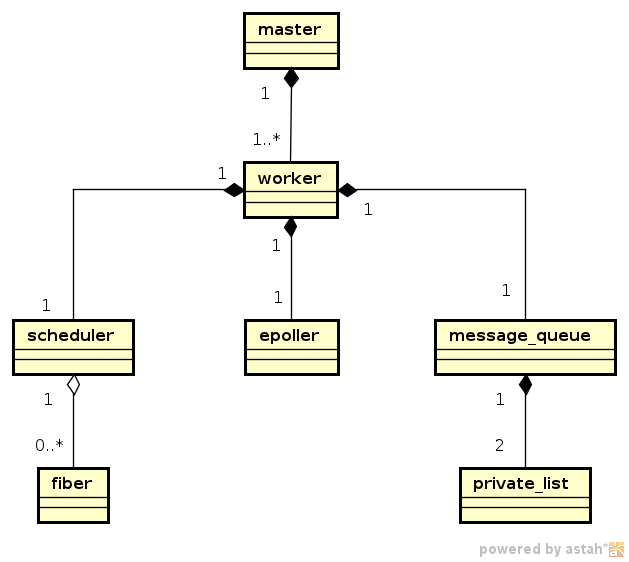
\includegraphics[scale=.6, angle=90]{libmixedOverview.png}
	\caption{Zależności pomiędzy pakietami biblioteki \code{libmixed}}
\end{figure}
\indent
	Biblioteka \code{libmixed} dostarcza implementację wątków hybrydowych, jednakże bez konieczności dokonywania zmian w~kodzie jądra systemu operacyjnego.
	Włókna są zaimplementowane w~sposób zbliżony do tego, jaki miał miejsce w~wypadku implementacji ULT w~bibliotece GNU Pth, jednakże to
	co różni ją od tamtej implementacji, to jej skalowalność: w~ramach jednej aplikacji możliwe jest zarządzanie wieloma grupami wątków.
	Inną istotną różnicą jest również brak udostępnienia dla użytkownika mechanizmów synchronizacji wątków, zaś w~zamian zagwarantowany
	jest wyłączny dostęp do wyróżnionych obiektów (klasy \code{fiber\dcolon resource}).
\par
%
\indent
	Biblioteka składa się z~czterech modułów:
	\begin{itemize}
		\item \code{libcoro} dostarcza podstawową dla włókien klasę \emph{koprocedur} wraz z~mechanizmami ich obsługi (m. in. obsługa  kontekstu
			wykonania koprocedury), jak również fabrykę, która wiąże dany kontekst z~obiektem klasy \code{coroutine}, lub wytwarza takowy;
		\item \code{libmanager} jest magazynem, który przechowuje konteksty wykonania dla obiektów klasy \code{coroutine};
		\item \code{libfiber} dostarcza klasę wątków, z~których korzysta użytkownik;
		\item \code{libscheduler}, który składa się z~nad-zarządcy (\code{ueber\_scheduler}) oraz bezpośrednich zarządców wątków dodawanych 
			przez użytkownika \linebreak (\code{userspace\_scheduler}).
	\end{itemize}
	Rysunek \ref{fig:libmixedoverview} pokazuje zależności pomiędzy poszczególnymi modułami biblioteki.
\par
%
\subsection{Moduł \code{libcoro}}
\label{sec:coroutine}
%
\indent
	Klasa \code{libcoro::abstract} jest \emph{interfejsem} dla koprocedury: informuje o~podstawowej funkcji, która musi być spełniona
	przez obiekt tej klasy. Tą funkcją jest niewątpliwie możliwość uruchomienia kodu koprocedury (wirtualna metoda \code{run()}).
	Klasa \code{libcoro::coroutine} dostarcza podstawowe mechanizmy potrzebne do obsługi koprocedury, m. in.:
	\begin{itemize}
		\item uruchomienie, wstrzymanie, wznowienie wykonania oraz terminacja koprocedury;
		\item obsługę kontekstu wykonania koprocedury: inicjalizacja, przełączanie pomiędzy kontekstami;
		\item przechwytywanie wyjątków.
	\end{itemize}
	Przeciążona metoda \code{run()} zawiera kod uruchamiany po uruchomieniu koprocedury,
	zaś wywołanie metody \code{start()} powoduje jej uruchomienie.
	Koprocedura może wstrzymać swoje działanie i~przekazać sterowanie programu do wywołującej ją koprocedury za pomocą metody \code{yield()}.
	Jeśli takie wywołanie miało miejsce, możliwe jest wznowienie jej działania poprzez ponowne wywołanie metody \code{start()}.
	Istnieje również możliwość przywrócenia kontekstu do stanu umożliwiającego jej ponowne uruchomienie od początku, taką funkcję spełnia
	metoda \code{rewind\procbr}.
	\begin{figure}[h!]
		\centering
		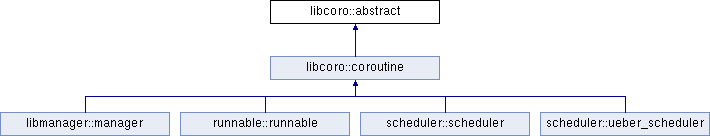
\includegraphics[scale=.5]{classlibcoroabstract.png}
		\caption{Klasa \code{libcoro\dcolon abstract} oraz jej klasy pochodne}
	\end{figure}
	Podczas działania aplikacji, można wyróżnić kilka stanów koprocedury:
	\begin{itemize}
		\item READY: koprocedura jest zainicjalizowana i~gotowa do uruchomienia; koprocedura jest w~tym stanie również po wykonaniu metody
			\code{yield\procbr};
		\item RUNNING: koprocedura w~trakcie działania;
		\item FINISHED: koprocedura zakończyła działanie;
		\item BLOCKED: koprocedura jest zablokowana;
		\item EXCEPTION, ERROR: wystąpił wyjątek (lub, odpowiednio - błąd) w~trakcie wykonania koprocedury;
		\item UNDEFINED: stan koprocedury niezdefiniowany (koprocedura nie powinna znaleźć się w~tym stanie).
	\end{itemize}
	\begin{figure}[h!]
		\centering
		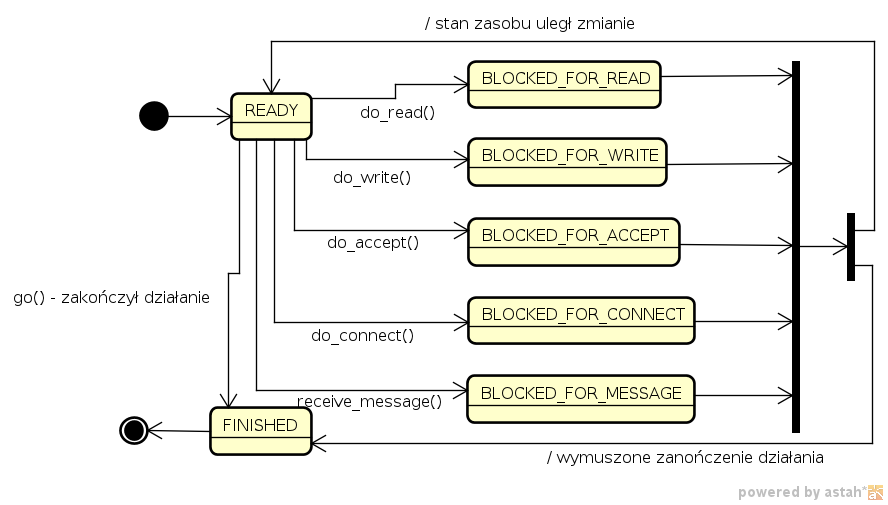
\includegraphics[scale=.7]{LibcoroStates.png}
		\caption{Stany koprocedury oraz dozwolone przejścia pomiędzy nimi}
	\end{figure}
\par
%
\indent
	Obsługa kontekstu wykonania koprocedury realizowana jest przy użyciu mechanizmu dostarczanego przez funkcje
	\code{getcontext()}/\code{swapcontext()}, dostępne w~każdym systemie zgodnym ze specyfikacją POSIX lub Single Unix Specification (SUS).
	Warto zauważyć, że jest to jeden ze sposobów obsługi kontekstu wykonania
	ULT w~bibliotece GNU Pth (inny sposób, wykorzystujący dalekie skoki \code{setjmp\procbr}/\code{longjmp\procbr} jest opisany w~\cite{Engelschall}).
\par
%
\indent
	Możliwe jest przechwytywanie wyjątków standardowych: \code{std\dcolon exception}. Informacja o~wystąpieniu wyjątku może być zignorowana,
	jak również zinterpretowana przez użytkownika w~następujący sposób:
	\begin{enumerate}
		\item Przeciążenie metody \code{on\_exception\procbr} w~obiekcie klasy \code{state\_controller}.
		\item Zgłoszenie obiektu jako kontrolera stanu koprocedury za pomocą metody \code{coroutine\dcolon set\_state\_controller\procbr}.
	\end{enumerate}
\par
%
\indent
	Aby wytworzyć koprocedurę gotową do uruchomienia, należy wytworzyć dla niej kontekst wykonania, lub też skorzystać z~już istniejącego
	kontekstu. Co więcej, zarówno kontekst jak i~koprocedura muszą być zainicjalizowane w~specyficzny sposób (ważna jest kolejność wykonania
	poszczególnych operacji). Obciążanie użytkownika odpowiedzialnością za wytworzenie działającej koprocedury może prowadzić do poważnych
	konsekwencji, np. błędów w~sekwencji wytwarzania koprocedury, czy też poważnymi zmianami w~aplikacji w~momencie zmiany implementacji
	kontekstu wykonania. Dlatego też implementacja kontekstu jest ukryta przed użytkownikiem, zaś koprocedury są wytwarzane przez funkcje znajdujące
	się w~module \code{libcoro\dcolon factory}. Przeciążona funkcja \code{assign\_coroutine\procbr} wiąże obiekt klasy \code{coroutine\procbr}
	z~kontekstem wykonania, który jest wytwarzany przez samą funkcję, bądź jest dostarczany wraz z~obiektem.
\par
%
\subsection{Moduł \code{libmanager}}
\indent
	Moduł \code{libmanager} jest odpowiedzialny za zarządzanie kontekstami wykonania koprocedur. Udostępnia następujące funkcje:
	\begin{itemize}
		\item pobranie kontekstu z~magazynu (\code{get\procbr});
		\item zwrócenie kontekstu do magazynu (\code{dispose\procbr}).
	\end{itemize}
	Obecnie moduł ten spełnia jedynie funkcje magazynu, nie posiada zaimplementowanych operacji zarządzania pamięcią.
	Operacje \code{get\procbr} oraz \code{dispose\procbr} nie są funkcjami \emph{reentrantnymi}.
	Mimo to, wydzielony magazyn dostarcza wygodnego mechanizmu do wytwarzania kontekstów wykonania koprocedur, zaś wydzielenie
	go jako osobnego modułu jest przydatne w~wypadku rozszerzania go o~wcześniej wspomniane funkcje.
\par
%
\subsection{Moduł \code{libfiber}}
\indent
	Moduł \code{libfiber} dostarcza podstawową klasę wątków używanych w~ramach biblioteki \code{libmixed}:
	klasa \code{fiber}, będąca klasą pochodną \code{coroutine}, zawiera dane potrzebne do identyfikacji
	konkretnego wątku, jak również dostarcza następujących mechanizmów:
	\begin{itemize}
		\item przesyłanie wiadomości (obiekty klasy \code{message}) pomiędzy wątkami za pomocą metod \code{send\procbr} oraz \code{receive\procbr}. 
			Ponieważ przesłanie wiadomości pomiędzy dwoma wątkami może wymagać pośrednictwa zarówno zarządcy przestrzeni użytkownika, jak również 
			nad\dywiz zarządcy, implementacja tego mechanizmu jest rozłożona pomiędzy te trzy komponenty. Szczegółowy opis mechanizmu przesyłania 
			wiadomości znajduje się w~rozdziale \ref{sec:scheduler}.
		\item \emph{Jacketing} urządzeń wejścia-wyjścia: metody \code{read\procbr} i~\code{write\procbr}, które, wywołane przez wątek, nie powodują
			zablokowania wywołania KLT, w~ramach którego wykonywany jest wątek. Podobnie jak w~wypadku implementacji mechanizmu przesyłania wiadomości,
			wymienione metody implementują część mechanizmu jacketingu związaną
			z~wątkiem, zaś obiekty klas opisanych w~rozdziale \ref{sec:scheduler} posiadają zaimplementowaną część tego mechanizmu, która jest wykonywana
			po stronie zarządcy (oraz nad\dywiz zarządcy).
	\end{itemize}
\par
%
\subsection{Moduł \code{libscheduler}}
\label{sec:scheduler}
\indent
	Moduł \code{libscheduler} zawiera dwie klasy planistów: \code{userspace\_scheduler} (ULS) oraz \code{ueber\_scheduler} (OLS).
	Klasa \code{userspace\_scheduler} jest odpowiedzialna za zarządzanie wątkami użytkownika w~obrębie jednego KLT.
	Do jej odpowiedzialności należy:
	\begin{itemize}
		\item wytworzenie oraz rejestracja gotowego wątku (metoda \code{spawn\procbr});
		\item przesyłanie wiadomości pomiędzy wątkami;
		\item jacketing urządzeń wejścia\dywiz wyjścia (pośredniczenie pomiędzy wątkiem a~OLS);
		\item szeregowanie wątków.
	\end{itemize}
	Powinnościami klasy \code{ueber\_scheduler} są:
	\begin{itemize}
		\item utworzenie \emph{pewnej} liczby wątków, każdy z~nich jest przyporządkowany  do obiektu klasy \code{userspace\_scheduler};
		\item nadzór nad ULS: rozpoczęcie pracy, zakończenie działania, przesyłanie żądań utworzenia nowego wątku;
		\item implementacja jacketingu: wykonanie wywołań systemowych, zarządzanie kolejką wątków oczekujących na I/O;
		\item pośrednictwo w~przekazywaniu wiadomości pomiędzy wątkami;
		\item obsługa zdarzeń systemowych oraz sygnałów.
	\end{itemize}
\par
%
\indent
	Komunikacja pomiędzy ULS a~OLS jest realizowana za pomocą potoków anonimowych (pipe).
\par
%
\indent
	Wszystkie wątki klasy \code{fiber} muszą spełniać warunek \emph{niezawodności}: muszą one przekazywać sterowanie do ULS w~\emph{rozsądnym} czasie
	(kończąc swoje działanie, lub poprzez operację \code{yield\procbr}).
\par
%
\indent
	Rozpoczęcie działania biblioteki jest równoznaczne z~wywołaniem metody \code{init\procbr} w~obiekcie klasy \code{ueber\_scheduler},
	zaś zakończenie działania OLS następuje po wykonaniu wszystkich wątków rozesłanych do posiadanych przez niego ULS.
\par
%
\remark
{
	We wtorek pojawi się opis mechanizmu wykrywania zakleszczeń.
}
\subsubsection{Wytworzenie wątku}
\indent
	Żądanie utworzenia (i~uruchomienia) wątku jest zgłaszane nad\dywiz planiście, zaś ten przekazuje je jednemu spośród ULS:
	\begin{itemize}
		\item metoda \code{ueber\_scheduler\dcolon spawn\procbr} przyjmuje jako argument wskaźnik do obiektu klasy \code{fiber}, który
			jest następnie przesyłany do ULS;
		\item po odebraniu żądania, ULS związuje kontekst z~przesłanym wątkiem i~dodaje go do kolejki wątków gotowych do uruchomienia.
	\end{itemize}
	\begin{figure}[h!]
		\label{fig:threadcreation}
		\centering
		\hspace*{-1cm}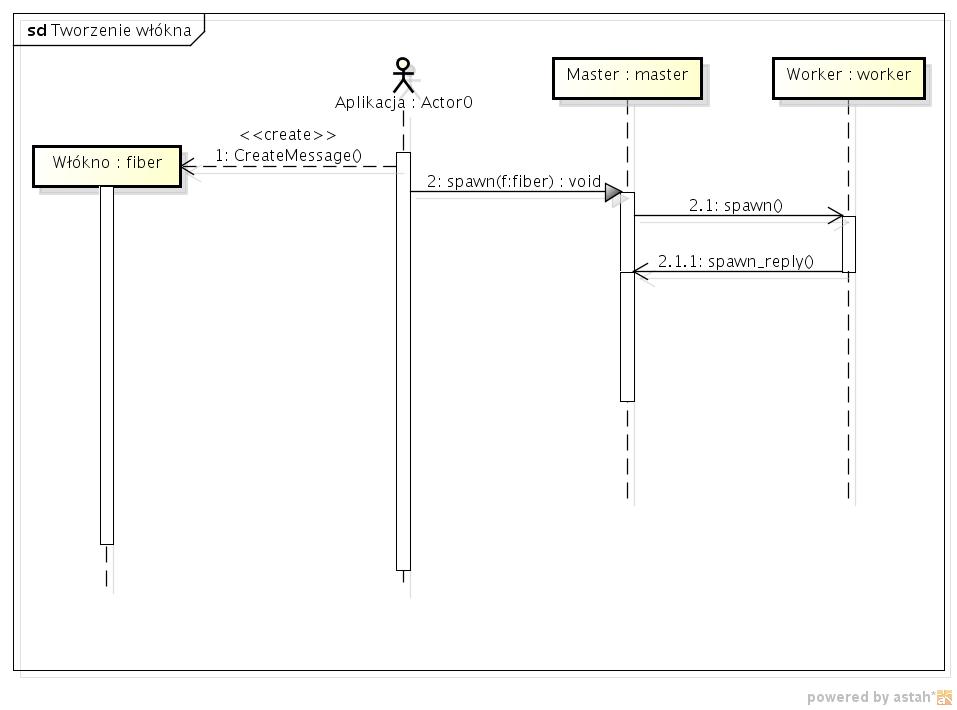
\includegraphics[scale=.6]{ThreadCreation.png}
		\caption{Wytworzenie wątku zarządzanego przez bibliotekę \code{libmixed}}
	\end{figure}
	Opisany sposób wytwarzania wątku posiada tę zaletę, że finalizacja tworzenia obiektu jest dokonywana w~miejscu rozpoczęcia jego wykonania.
	Co więcej, wątek jest w~stanie \emph{wędrować} pomiędzy zarządzającymi nim planistami (zarówno ULS, jak też może być przechowywana przez
	OLS).
\par
%
\subsubsection{Przesyłanie wiadomości pomiędzy wątkami}
\indent
	Mechanizm przesyłania wiadomości pomiędzy wątkami spełnia następujące założenia:
	\begin{itemize}
		\item wysyłanie i~odbiór wiadomości mogą blokować działanie wątku, jednakże nie mogą blokować działania żadnego planisty biorącego udział
			w~komunikacji międzywątkowej;
		\item mechanizm ma być przezroczysty dla wątku: bez względu na wzajemne położenie wątków (zarządzanie przez tego samego planistę lub
			przez dwóch innych planistów), z~perspektywy wątku komunikacja pomiędzy nimi odbywa się tak samo.
	\end{itemize}
	Rysunek \ref{fig:interthreadmessaging1} oraz rys.~\ref{fig:interthreadmessaging2} przedstawiają możliwe scenariusze wędrówki wiadomości 
	pomiędzy dwoma wątkami.
	\begin{figure}[h!]
		\label{fig:interthreadmessaging1}
		\centering
		\hspace*{-1cm}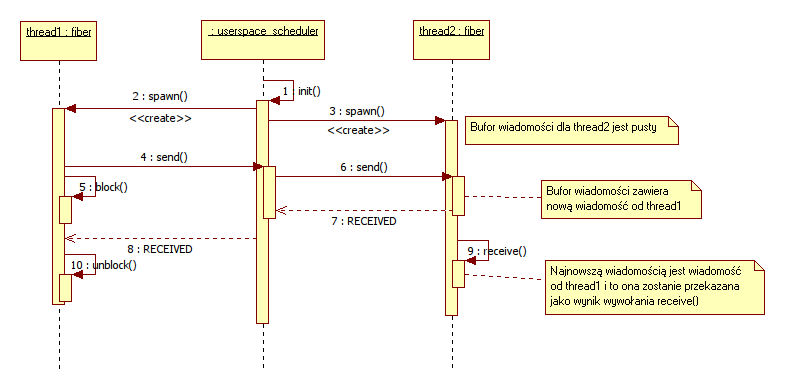
\includegraphics[scale=.6,angle=90]{InterThread1.png}
		\caption{Wysłanie wiadomości z~wątku thread1 do wątku thread2 w~ramach tego samego ULS}
	\end{figure}
	\begin{figure}[h!]
		\label{fig:interthreadmessaging2}
		\centering
		\hspace*{-1cm}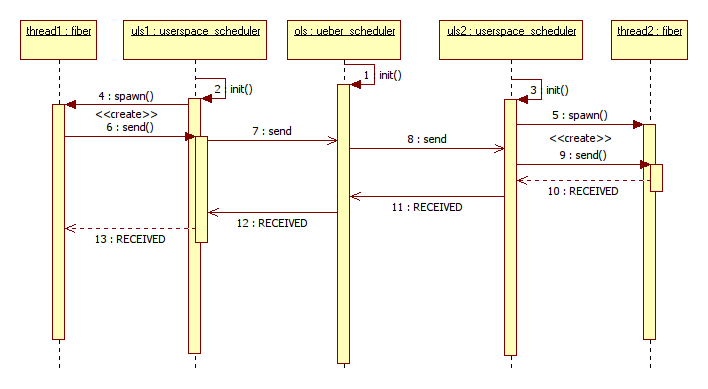
\includegraphics[scale=.6,angle=90]{InterThread2.png}
		\caption{Wysłanie wiadomości z~wątku thread1 do wątku thread2 w~ramach tego samego ULS}
	\end{figure}
	W~obecnej implementacji:
	\begin{itemize}
		\item operacja \code{send\procbr} powoduje zablokowanie wątku wysyłającego wiadomość; po dostarczeniu wiadomości do odbiorcy, 
			sterowanie powraca do wątku, \code{send\procbr} podaje wynik wysłania wiadomości;
		\item operacja \code{receive\procbr} powoduje sprawdzenie bufora wiadomości dla danego wątku; jeśli jest niepusty, \code{receive\procbr}
			przekazuje jako wynik pierwszą wiadomość z~bufora.
	\end{itemize}
\par
%
\subsubsection{Jacketing urządzeń wejścia\dywiz wyjścia}
\indent
	Implementacja dostarcza nieblokujący dostęp do systemu plików oraz udostępnia nieblokujące gniazda sieciowe.
	Podobnie jak w~wypadku komunikacji międzywątkowej, wątek dokonujący odczytu lub zapisu do takiego zasobu, jest blokowany,
	a~nadzorujący go ULS przesyła żądanie do OLS.
	To właśnie w~nad\dywiz zarządcy znajduje się część implementacji, w~której znajdują się (nieblokujące) wywołania systemowe,
	zaś wyniki poszczególnych operacji na zasobach systemowych są przesyłane do odpowiednich ULS.
\par
%
\indent
	Obecnie dostępne są dwa rodzaje zasobów systemowych: plik \linebreak (\code{scheduler\dcolon file}) oraz gniazdo (\code{scheduler\dcolon socket}).
	Posiadają one metody do odczytu (\code{read\procbr}) oraz zapisu (\code{write\procbr}).
\par
%
\section{Analiza rozwiązania}
\label{sec:analysis}
\subsection{Kryteria oceny}
\indent
	Użyteczność implementacji opisanej w~poprzednim rozdziale można określić za pomocą porównania jej wydajności z~szeroko rozpowszechnionymi
	implementacjami wątków. Obecnie nie jest dostępna implementacja wątków, która spełniała by następujące wymogi:
	\begin{itemize}
		\item zaimplementowana w~C++;
		\item nie wymaga zmian w~jądrze systemu;
		\item model N:M.
	\end{itemize}
	Ponieważ bieżąca implementacja w~części odpowiedzialnej za KLT korzysta implementacji Pthreads, zaś część implementująca ULT
	jest wzorowana na rozwiązaniach stosowanych w~bibliotece GNU Pth, naturalnym wyborem do testów porównawczych jest
	użycie tych implementacji wątków.
\par
%
\subsection{Testy}
\indent
	Porównanie implementacji z~istniejącymi obejmuje następujące właściwości biblioteki:
	\begin{itemize}
		\item maksymalna liczba wątków do uruchomienia w~ramach jednej aplikacji;
		\item czas wykonania \emph{pustych} wątków (ang. \emph{null fork});
		\item czas wykonania przeplatających się wątków (w~przypadku \code{libmixed} polega to na zastosowaniu operacji \code{yield\procbr});
		\item operacje na współdzielonych zasobach (np. inkrementacja współdzielonego licznika);
		\item komunikacja międzywątkowa;
		\item szybkość działania na plikach;
		\item wydajność gniazd sieciowych (implementacja prostego serwera).
	\end{itemize}
\par
%
\subsection{Wyniki}
\section{Podsumowanie}
\label{sec:summary}
\subsection{Narzędzia}
\indent
\remark
{
	\begin{itemize}
		\item GCC
		\item Libtool
		\item GNU Make
		\item GNU GDB, DDD
		\item Valgrind (użyte narzędzia)
	\end{itemize}
}
\par
\subsection{Możliwe kierunki rozwoju}
%
\newpage
\rhead{\empty}
%\pagestyle{plain}
\bibliography{bibliography}
\begin{comment}
\section*{Indeks}
\printindex
\end{comment}
\end{document}
